\chapter{Dinamica del punto materiale} %2
%-------------------------------------------------------------------------------------------
La dinamica, è la branca della fisica che studia le cause che generano
o variano lo stato di moto di un corpo.
\section*{Leggi di Newton}
\begin{enumerate}
    \item Prima legge di Newton (Principio d'inerzia):
    Un corpo non soggetto a forze esterne non subisce cambiamenti di velocità,
    ovvero resta in quiete o in moto rettilineo uniforme.
    \item Seconda legge di Newton:
    La somma delle forze che agiscono su un corpo è proporzionale
    all'accelerazione del corpo stesso, mediante un coefficiente chiamato
    massa inerziale.\\
    \begin{equation}
        \boxed{\vec F = m\vec a}
    \label{eq:newt2law}
    \end{equation}
    \item Terza legge di Newton (Principio di azione e reazione): Se un
    corpo $A$ esercita una forza $F$ su un corpo $B$, allora $B$ esercita
    una forza $-F$ su $A$.
    Quindi la forza ha le unità di misura di una massa per una lunghezza
    per un tempo alla meno due.    
\end{enumerate}
L'unità di misura della forza è il Newton $(N)$ ed è definito come
$\sx Kg\frac m{s^2}\dx$. 
$$ \vec F = m\vec a = m\frac{d\vec v}{dt} = m\frac{d^2\vec x}{dt^2}\quad\quad
\left[F\right] = M\cdot L\cdot T^{-2} \seg 1N = 1 Kg\cdot\frac m{s^2}$$

\section{Quantità di moto}
%---------------------------------------------------------------------------
Una grandezza molto importante che si introduce in dinamica è la quantità
di moto o impulso o momento (lineare). La quantità di moto di un corpo è
definita come il prodotto tra la sua massa e la sua velocità, dunque nel
sistema internazionale si misura in chilogrammi per metro al secondo.
\begin{equation}
    \boxed{\vec p = m\vec v}\quad\quad \sss p\ddd = M\cdot L\cdot T^{-1}
\label{eq:pulse_def}
\end{equation}
Nel caso in cui la massa dell'oggetto sia costante nel tempo, ovvero nella
maggior parte dei casi che incontreremo, derivando l'impulso rispetto al
tempo otterremo che:
\begin{equation}
    \frac{d\vec p}{dt} = \frac d{dt}\sx m\vec v\dx =
    m\frac{d\vec v}{dt} =\vec F
\end{equation}
Quindi la seconda legge di Newton nel caso più generale, identifica la
forza come la derivata temporale della quantità di moto.
\begin{equation}
    \boxed{\vec F = \frac{d\vec p}{dt}}
\label{eq:newt2law_p}
\end{equation}
\subsection{Teorema dell'impulso}
Integrando l'equazione (\ref{eq:newt2law_p}) possiamo ricavare la variazione della
quantità di moto tra istante finale e istante iniziale che chiameremo impulso $(\vec J)$.
\begin{equation}
    \vec F = \frac{d\vec p}{dt}\seg \int_{t_0}^tdt'\frac{d\vec p}{dt'} =
    \int_{t_0}^tdt'\vec F\seg \vec p_{(t)} - \vec p_{\sx t_0\dx} =
    \int_{t_0}^tdt'\vec F
\end{equation}
\begin{equation}
    \boxed{\vec J = \int_{t_0}^tdt'\vec F_{(t')}}
\label{eq:pulse_theorem}
\end{equation}
\\
Per il teorema della media, il valor medio della forza  è proprio il rapporto tra variazione di quantità di moto e intervallo di tempo.
\begin{equation}
\vec F_m = \frac1{t-t_0}\int_{t_0}^tdt'\vec F = \frac{\Delta\vec p}{\Delta t}
\end{equation}
\begin{itemize}
    \item Se $\vec F$ è costante nel tempo allora:
    \begin{equation}
        \vec J = \vec F\Delta t\seg\Delta\vec p = \vec J \seg\Delta\vec v
        = \frac{\vec J}m
    \end{equation}
    \\\item Se $\vec F$ è nulla allora:
    \begin{equation}
        \Delta\vec p = 0\seg\vec p_{(t)} = cost
    \end{equation}
    In assenza di forze applicate la quantità di moto di un corpo si conserva.
\end{itemize}
\section{Forze}
%---------------------------------------------------------------------------
Se su un corpo agiscono più forze, diremo che il corpo è in equilibrio
statico se e solo se la risultante delle forze (la somma) è nulla.\\
Supponiamo di avere un corpo soggetto ad $n$ forze, se chiamiamo la
forza $i$-esima: $\vec F_i$, la risultante sarà:

\begin{equation}
    \vec F = \sum_{i=1}^n\vec F_i =  \sum_{i=1}^n m\vec a_i =
    m \sum_{i=1}^n \vec a_i\quad\mbox{eq. statico}\quad\Leftrightarrow
    \quad\vec F = \vec 0
\label{eq:forces:superposition}
\end{equation}

\subsection{Forza di reazione vincolare}
Ogni volta che un corpo soggetto ad una forza incontra un vincolo,
quest'ultimo esercita per il principio di azione e reazione un forza
uguale e opposta, in modo tale da bilanciare la forza applicata.
La forza di reazione vincolare è chiamata anche forza di reazione normale,
dato che è ortogonale al vincolo ed infatti è indicata con la lettera $\vec N$.
\begin{figure}[htbp]
    \begin{center}
        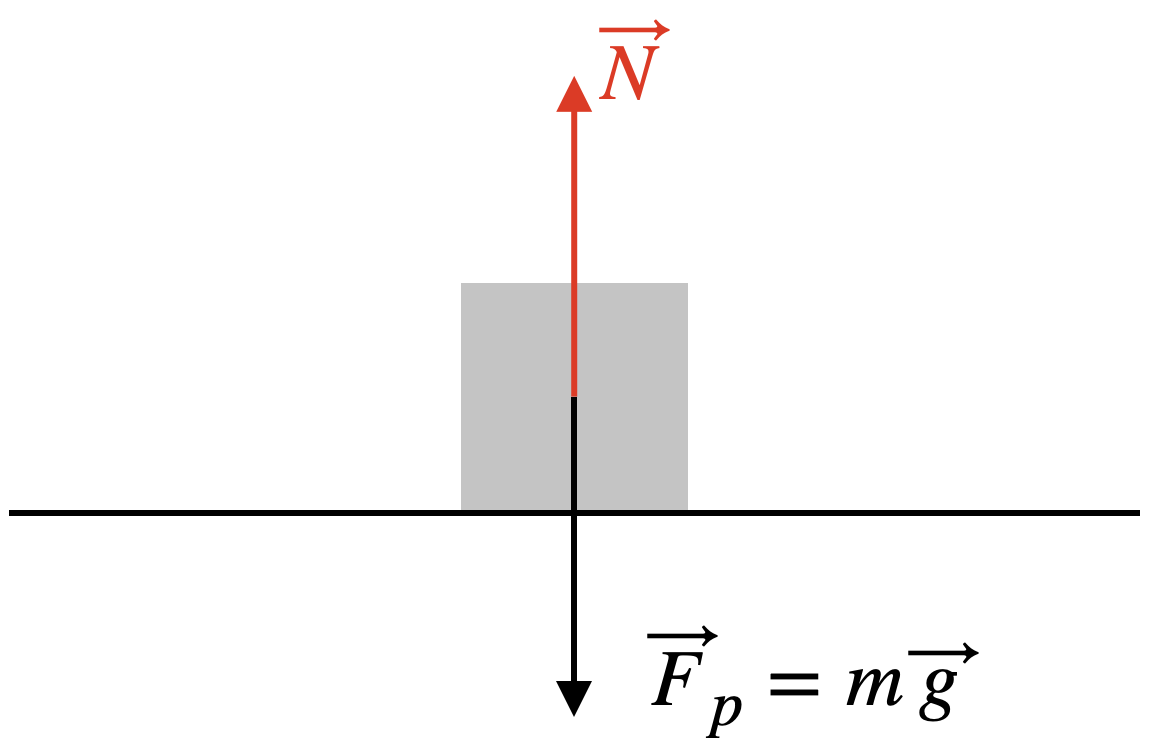
\includegraphics[width=7cm]{images/NP.png}
        \caption{Corpo in equilibrio soggetto alla forza peso ed  alla
        reazione vincolare.}
    \end{center}
\label{fig:forces:vincolar_reaction}
\end{figure}
\\
In questo caso abbiamo solo due forze, la forza peso e la forza di reazione
vincolare e sono entrambe dirette lungo la stessa direzione, ma di verso
opposto.

\begin{equation}
    \vec N + \vec F_p = \vec 0 \seg N - F_p = N - mg = 0 \seg \boxed{N = mg}
\label{eq:forces:vincolar_reaction}
\end{equation}
\\
\begin{figure}[htbp]
\center
        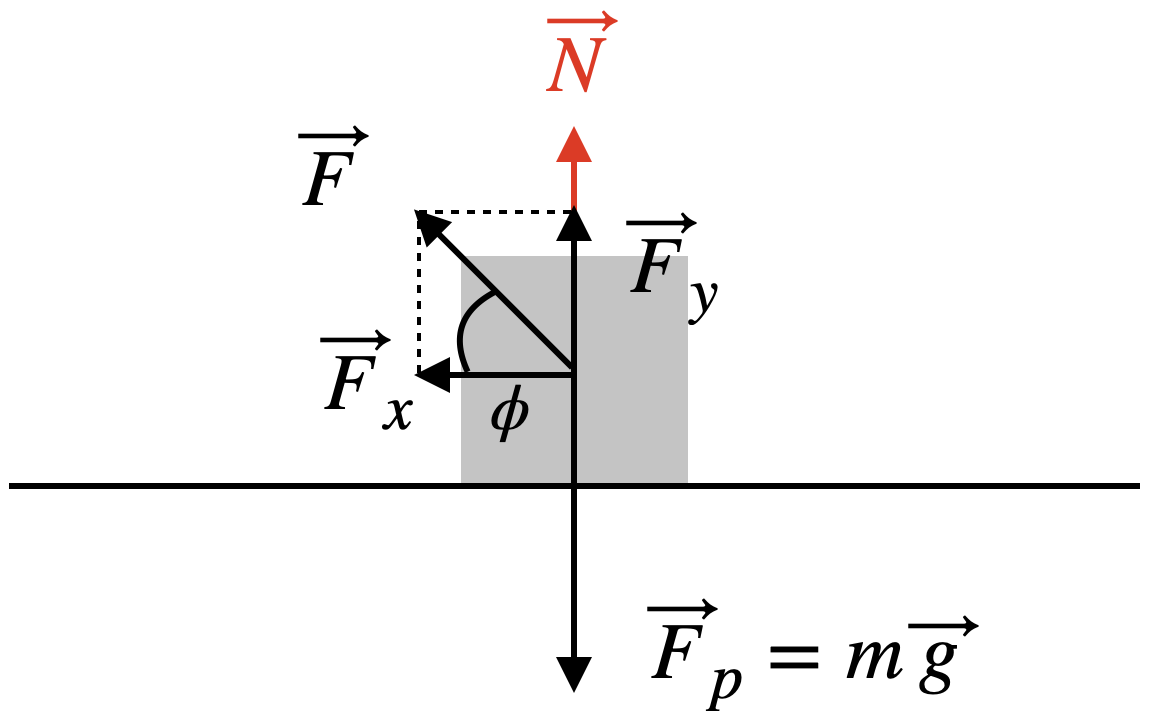
\includegraphics[width=7cm]{images/NPF.png}
        \caption{Corpo soggetto alla forza peso, alla forza $\vec F$ ed alla
        reazione vincolare.}
        \label{fig:vincolar_reaction_2}
\end{figure}
\\
Nella situazione rappresentata in figura (\ref{fig:vincolar_reaction_2}),
notiamo che l'aggiunta di una terza forza nel sistema modifica l'intensità
di $\vec N$. Per prima cosa bisogna scomporre lungo l'asse $x$ ed $y$ la
forza $\vec F$.

\begin{equation}
    \vec F = \vec F_x + \vec F_y = F_x\hat\imath + F_y\hat\jmath\seg 
    \begin{cases}
        F_x = -F\cos\phi <0\\
        F_y = F\sin\phi>0
    \end{cases}
\end{equation}
\\
Adesso procediamo con il calcolo scrivendo le equazioni di Newton.

\begin{equation}
    x:\quad F_x = m\ddot x\qquad
    y:\quad N-mg+F_y = m\ddot y = 0
\end{equation}
\\
\begin{equation}
    \mbox{Ne segue che la reazione vincolare è:}\quad \boxed{N = mg -F\sin\phi}
\end{equation}
\\
Per quanto riguarda l'asse $x$, c'è solo la componente orizzontale di
$\vec F$ che agisce sul corpo, dunque, supponendo $\phi$ ed il modulo della
forza $F$ costanti nel tempo e $\phi\ne\frac\pi2$, il corpo si muove di moto
uniformemente accelerato lungo la direzione negativa dell'asse $x$.
Con accelerazione pari a: $a = \frac{F_x}{m} = -\frac Fm\cos\phi$.

\subsection{Forze d'attrito}
Per capire cosa si una forza d'attrito consideriamo ancora il caso raffigurato
in figura (\ref{fig:vincolar_reaction_2}). La conclusione a cui siamo
giunti, ovvero che il corpo si
muove di moto uniformemente accelerato, implica l'aver considerato che non ci
sia interazione tra il corpo ed il vincolo, lungo la direzione $x$.
Inoltre è stato completamente trascurato l'effetto dell'aria sul corpo
durante il moto.
In realtà esistono tre tipi di forze, forze d'attrito, che migliorano la
descrizione del problema precedentemente trattato.\\
Le forze d'attrito radente statico e dinamico e la forza d'attrito viscoso.
\subsubsection{Attrito statico}
La forza d'attrito radente statico è la responsabile del fatto che un corpo,
posto su un piano, ha bisogno di una certa forza iniziale per cominciare il
moto. Se questo tipo di forza non esistesse basterebbe un forza piccola a
piacere per mettere un corpo in moto.\\
La forza d'attrito statico è caratterizzata dal fatto che ha un valore
variabile, da un minimo di zero, quando non si applica nessuna forza esterna,
ad un massimo che segneremo con $F_s$.
\\Dunque applicando gradualmente una forza esterna, avremo che la forza
d'attrito aumenterà anch'essa in modo graduale, bilanciando perfettamente
la forza esterna, fino al suo valore massimo.\\
Quindi ritornando al caso della figura (\ref{fig:vincolar_reaction_2})
il corpo inizia a muoversi solo se $F\cos\phi > F_s$.

\begin{equation}
    F_s = \mu_sN
\label{eq:forces:static}
\end{equation}
\\
\begin{equation}
    -F\cos\phi + F_s = -F\cos\phi + \mu_s N < 0\seg F\cos\phi >
    \mu_s\sx mg - F\sin\phi\dx
\end{equation}
\\
Dove $\mu_s$ è chiamato coefficiente d'attrito statico.
Ora supponendo di mantenere fissato l'angolo $\phi$ calcoliamo quali
valori deve assumere $F = \left|\vec F\right|$ per mettere in moto l'oggetto.

\begin{equation}
    F > \frac{\mu_s}{\mu_s\sin\phi+\cos\phi}mg
\end{equation}

\subsubsection{Attrito dinamico}
L'attrito dinamico invece entra in gioco proprio quando la forza esterna
supera il valore della forza d'attrito massima. La forza d'attrito dinamico
è una forza costante diretta in direzione opposta a quella della velocità
dell'oggetto.\\
Quindi una volta che la forza esterna supera il valore di $F_s$,
la forza d'attrito statico si annulla e si "attiva" la forza d'attrito dinamico.

\begin{equation}
    \vec F_d = -\mu_dN\hat u_v
\label{eq:forces:dynamic}
\end{equation}
\\
Supponiamo di avere una forza che soddisfi la (\ref{eq:forces:dynamic})
ne segue che:

\begin{equation}
    -F\cos\phi + \mu_dN = m\ddot x \seg \ddot x =
    \mu_dg-\frac Fm\sx\mu_d\sin\phi + \cos\phi\dx
\end{equation}
\\
L'accelerazione del corpo subisce una modifica. Trascurare l'attrito
significa considerare $\mu_{s,d}\ll 1$, ed infatti in questa approssimazione
riotteniamo il caso discusso nel paragrafo precedente, ovvero:

\begin{equation}
    F>0\quad\quad \ddot x = -\frac Fm\cos\phi
\end{equation}
\\
Un'ultima cosa da dire è che il coefficiente d'attrito statico $\mu_s$ è
sempre maggiore del coefficiente d'attrito dinamico $\mu_d$, infatti è più
facile mantenere in moto il corpo, piuttosto che spostarlo dalla sua
posizione di quiete.

\subsubsection{Attrito viscoso}
La forza di attrito viscoso è dovuto alla resistenza che oppone un fluido
quando un corpo è in movimento al suo interno. Se il fluido è in regime
laminare (non turbolento) la forza di attrito viscoso può essere stimata
con la seguente formula.

\begin{equation}
    \vec F_v = -b\vec v
\label{eq:forces:viscous}
\end{equation}
\\
Dove $b$ è il coefficiente di attrito viscoso ed è collegato alle proprietà
geometriche del corpo ed alla viscosità del fluido in questione.

\begin{equation}
    b = k\eta
\label{eq:forces:viscous_coefficient}
\end{equation}
\\
Dove $\eta$ è la viscosità del fluido, ha le dimensioni di una pressione per
un tempo $(Pa \cdot s) =(N\cdot m^{-2}\cdot s)$. Mentre $k$ è il fattore
geometrico che dipende dalla forma del corpo ed è misurato in metri, ad
esempio per una sfera $k = 6\pi R$.
Se sul corpo non agiscono altre forze oltre a quella d'attrito viscoso,
allora abbiamo anche un'accelerazione proporzionale alla velocità e dunque
un moto smorzato esponenzialmente, come quello incontrato nel paragrafo (\ref{section:MRSE}).

\begin{equation}
    \vec F_v = -k\eta\vec v = m\vec a \seg
    \vec a = -\frac{k\eta}m\vec v =-\beta \vec v 
\end{equation}
\\
È interessante considerare il caso di caduta libera in presenza di attrito
viscoso. Scegliamo un sistema di riferimento unidimensionale rivolto verso
il basso, e lasciamo cadere un oggetto a partire dall'origine.
\begin{figure}[htbp]
    \begin{center}
        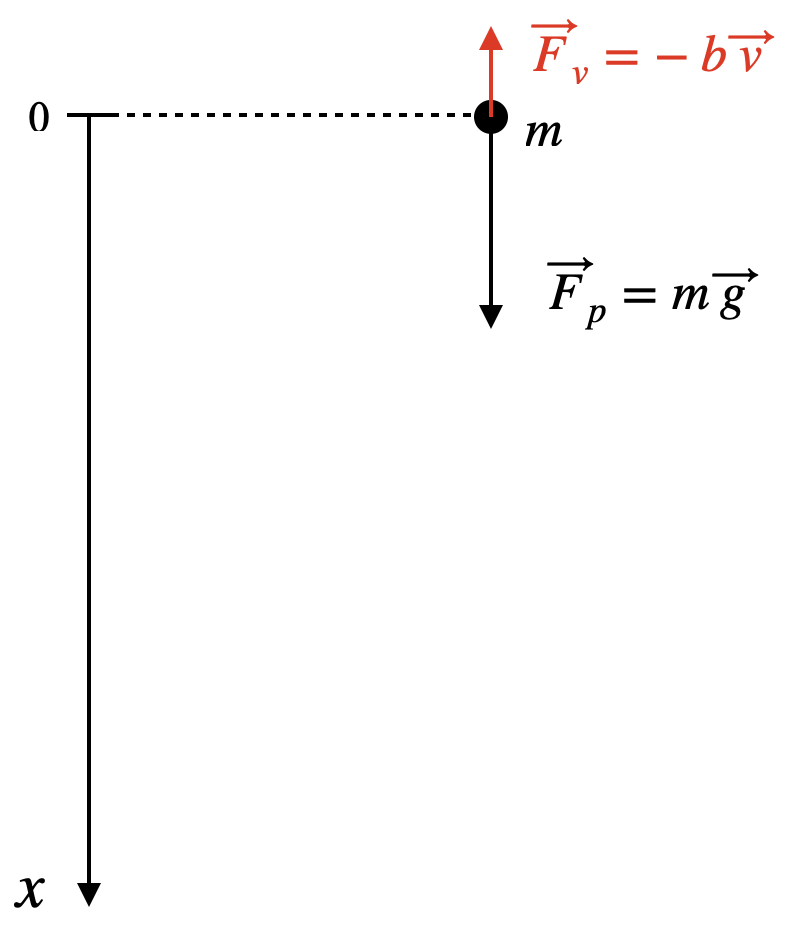
\includegraphics[width=7cm]{images/cadlibera.png}
        \caption{Corpo di massa $m$ soggetto alla forza peso ed
        alla forza di attrito viscoso.}
\end{center}
\label{fig:forces:freefall}
\end{figure}
\\
Quindi scrivendo la somma delle forze che agiscono su $m$ otterremo:

\begin{equation}
    mg - bv = m\dot v \seg \dot v = g - \frac{b}{m}v
\end{equation}
\\
Ora definiamo un tempo caratteristico del sistema, che chiameremo $\tau$.
Questo fattore determina una scala temporale del moto. La regione in cui
$t\gg\tau$ è chiamata regime, mentre la zona in cui $t\gg\tau$ è chiamata
transiente.

\begin{equation}
    \boxed{\tau \coloneqq \frac{m}{b} = \frac1\beta}
\label{eq:forces:time_constant}
\end{equation}
\\
Andiamo ora a ricavare la velocità in funzione del tempo.

\begin{equation}
    \dot v = g - \frac bmv = g - \frac v\tau = -\frac1\tau\sx v - g\tau\dx
    \seg \frac{\dot v}{v -g\tau} = -\frac1\tau
\end{equation}
\\
\begin{multline}
   \int_0^{v_{(t)}}\frac{d v}{v -g\tau} = -\int_0^t\frac{dt'}\tau\seg
   \ln\sss 1 - \frac{v_{(t)}}{g\tau}\ddd = -\frac t\tau\seg
   \\\seg\boxed{v_{(t)} = g\tau\sx1-e^{-\frac t\tau}\dx}
\label{eq:forces:viscous_v}
\end{multline}
\\
Integrando nuovamente si ottiene l'equazione del moto:

\begin{equation}
    x_{(t)} = g\tau\int_0^tdt'\sx1-e^{\frac{-t'}\tau}\dx \seg
    \boxed{x_{(t)} = g\tau\sss t + \tau\sx e^{-\frac t\tau} - 1\dx\ddd}
\label{eq:forces:viscous_x}
\end{equation}
\\
\begin{figure}[htbp]
\center
        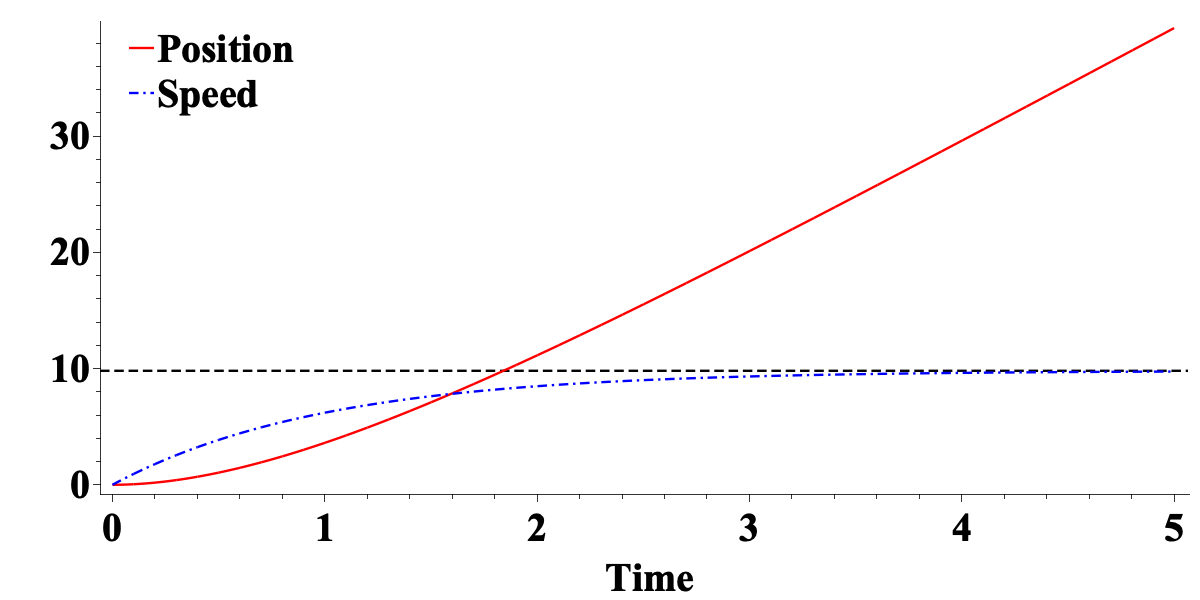
\includegraphics[width=13cm]{images/freefallXV.png}
        \caption{Spazio percorso (rosso) e velocità (blu) di un corpo in
        caduta libera con attrito viscoso. La linea orizzontale tratteggiata
        rappresenta il valore asintotico (a regime) della velocità.
        L'asse delle ascisse rappresenta il tempo in unità di $\tau$.}
\label{fig:forces:freefall:curves}
\end{figure}
\\
Il valore a regime di $v_{(t)}$ si calcola facendo il limite per
$t\gg\tau\seg$

\begin{equation}
    v_\infty\coloneqq v_{\sx t\gg\tau \dx} = g\tau
\label{eq:forces:viscous_vlim}
\end{equation}
\\
La velocità tende a diventare costante in quanto la forza d'attrito tende a
bilanciare la forza peso dunque il corpo tenderà a muoversi di moto
rettilineo uniforme.\\
Se invece sviluppiamo sia $x_{(t)}$ che $v_{(t)}$ per $t\ll\tau$,
possiamo osservare che l'effetto della forza d'attrito è ancora troppo
piccolo e quindi le curve posso essere approssimate con le equazioni della
caduta libera senza attrito.\\
Le leggi orarie della posizione e della velocità, ed anche la velocità di regime
sono rappresentate in figura (\ref{fig:forces:freefall:curves}). Nelle figure
(\ref{fig:freefall_approx_x}) e (\ref{fig:freefall_approx_v})
abbiamo messo in risalto la differenza tra le soluzioni con attrito e quelle
senza attrito.

\begin{figure}[htbp]
    \center
    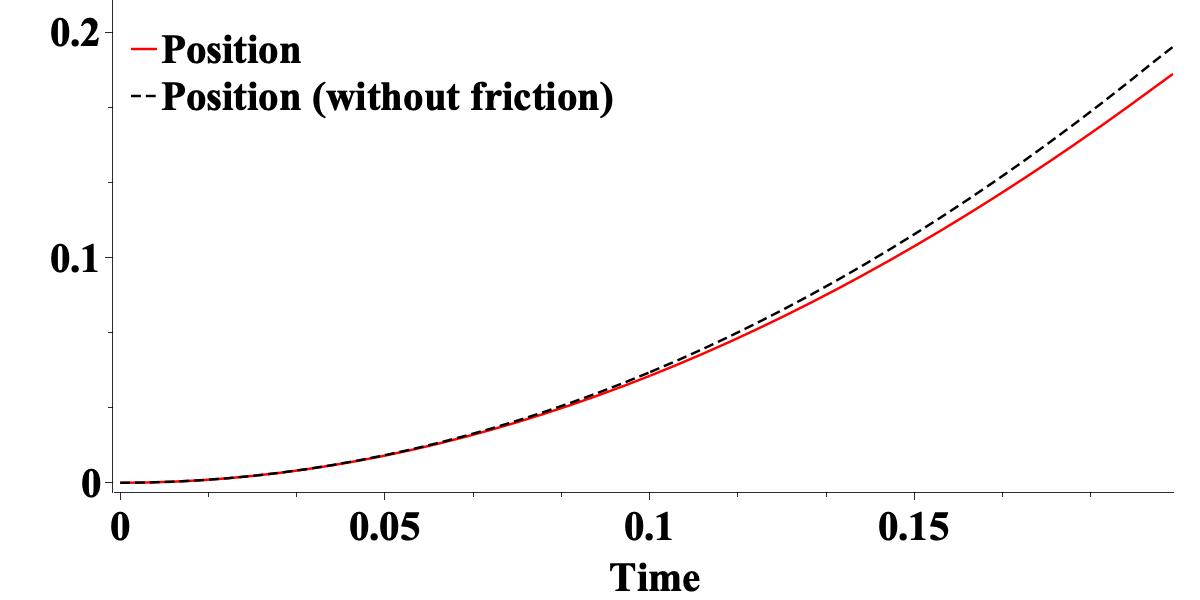
\includegraphics[width=13cm]{images/freefallX.png}
    \caption{Approssimazione per piccoli tempi, la curva nera è l'equazione
    della posizione in funzione del tempo in caduta libera senza attrito:
    $x_{(t)} = \frac12gt^2$}
\label{fig:freefall_approx_x}
\end{figure}

\begin{figure}[htbp]
\center
    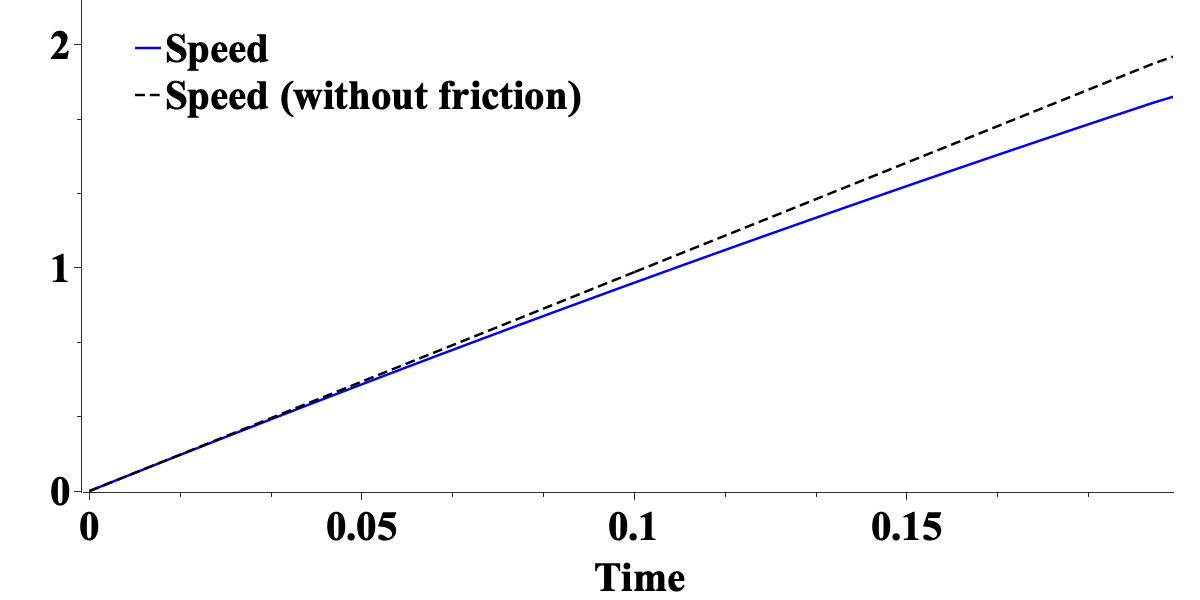
\includegraphics[width=13cm]{images/freefallV.png}
    \caption{Approssimazione per piccoli tempi, la curva nera è l'equazione
    della velocità in funzione del tempo in caduta libera senza attrito:
    $v_{(t)} = gt$}
\label{fig:freefall_approx_v}
\end{figure}

\subsection{Forza elastica}
La forza elastica è una forza di richiamo generata da una molla, quando viene
discostata dalla sua posizione di equilibrio. Essa è proporzionale alla
contrazione/dilatazione effettuata.\\ Quindi se supponiamo di avere un un
punto collegato ad una molla in posizione iniziale $\vec x_0$, e lo spostiamo
fino al punto $\vec x$, allora la forza elastica sarà:

\begin{equation}
    \vec F_e = -k\sx\vec x-\vec x_0\dx = -k\Delta x\cdot\hat u_x
\end{equation}
\\
\begin{figure}[htbp]
    \begin{center}
        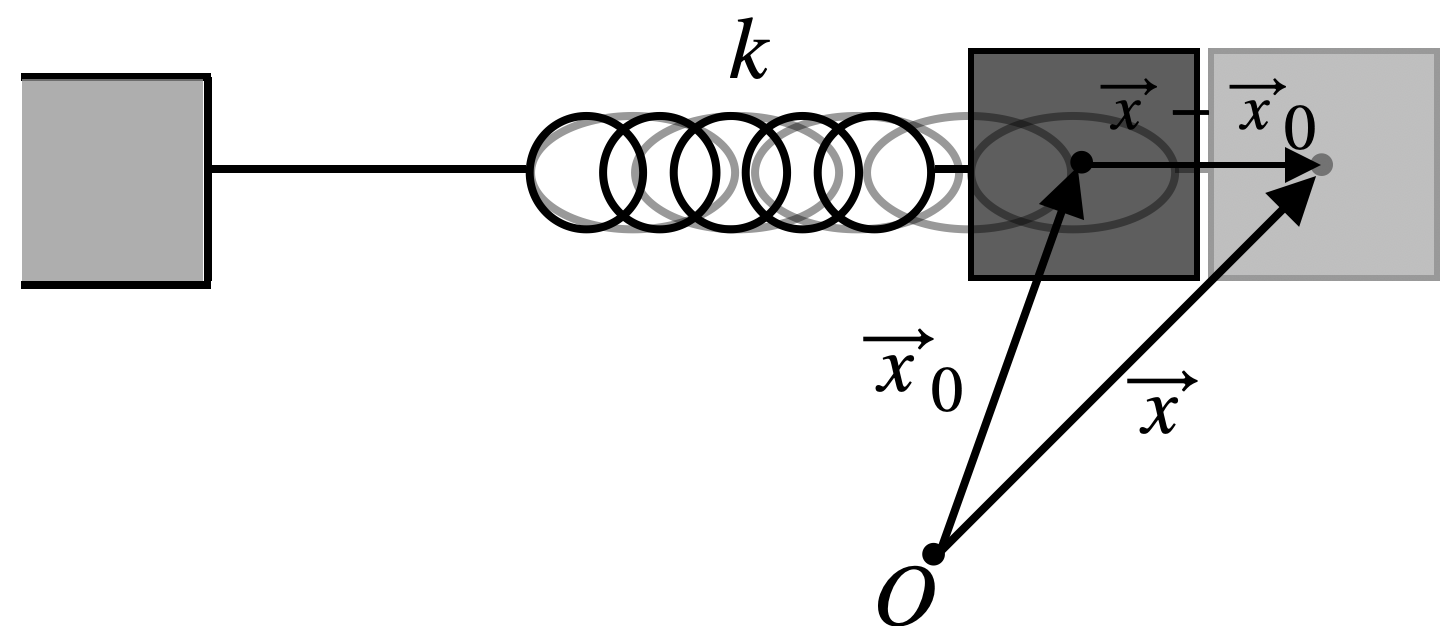
\includegraphics[width=10cm]{images/molla.png}
        \caption{Rappresentazione dell'elongazione di una molla rispetto
        alla sua posizione di riposo.}
\end{center}
\label{fig:forces:elastic}
\end{figure}
\\
La costante elastica $k$ è caratteristica della molla ed è misurata in
$\frac Nm$. Se studiamo il caso dinamico in cui un corpo è soggetto alla
sola forza elastica otterremo che:

\begin{equation}
    F_x = m\ddot x = -kx \seg \boxed{\ddot x +\frac km x = 0}
\label{eq:forces:elastic_ODE}
\end{equation}
\\
È l'equazione differenziale dell'oscillatore armonico con
$\omega = \sqrt{\frac km}$ e periodo $T =2\pi\sqrt{\frac mk}$.
La soluzione sarà come la (\ref{eq:MA}), possiamo utilizzare la funzione
coseno in quanto il punto parte da una posizione pari a $\Delta x$:

\begin{equation}
    x_{(t)} = \Delta x \cos\sx \sqrt{\frac km}t\dx
\label{eq:forces:elastic_x}
\end{equation}
\\
In realtà non è necessaria la presenza di una molla per avere una forza
elastica, e quindi questo tipo di moto, ma qualsiasi sistema fisico in cui è
presente una forza come quella in (\ref{eq:forces:elastic_ODE}) è
riconducibile ad un oscillatore armonico semplice.
\section{Piano inclinato}
%---------------------------------------------------------------------------
Vogliamo studiare il problema di un punto materiale di massa $m$ in caduta
libera, lungo un piano inclinato con pendenza $\theta$. Studieremo prima il
caso senza attrito e poi il caso con attrito, trascureremo in entrambi i
casi l'attrito viscoso con l'aria. \\
Scegliamo un sistema di riferimento con l'asse $x$ parallelo al piano e
l'asse ortogonale ad esso, come mostrato in figura (\ref{fig:Iplain&pendulum:Iplain}).
\\ Nel caso senza attrito le forze in gioco sono: la forza peso diretta in
direzione verticale e scomponibile in $\vec F_{px}$ ed $\vec F_{py}$, e la
forza di reazione vincolare diretta lungo la direzione positiva dell'asse $y$.
Dunque avremo che:
\begin{equation}
    x:\quad mg\sin\theta = m\ddot x\quad\quad y: \quad N - mg\cos\theta = 0
\end{equation}
$$\Downarrow$$
\begin{equation}
    \begin{cases}
        a_x = g\sin\theta\\
        N = mg\cos\theta
    \end{cases}
    \seg x_{(t)} = \frac12 g\sin\theta\cdot t^2
\end{equation}
Si ha un moto uniformemente accelerato con accelerazione $g\sin\theta$.
\begin{figure}[htbp]
    \begin{center}
        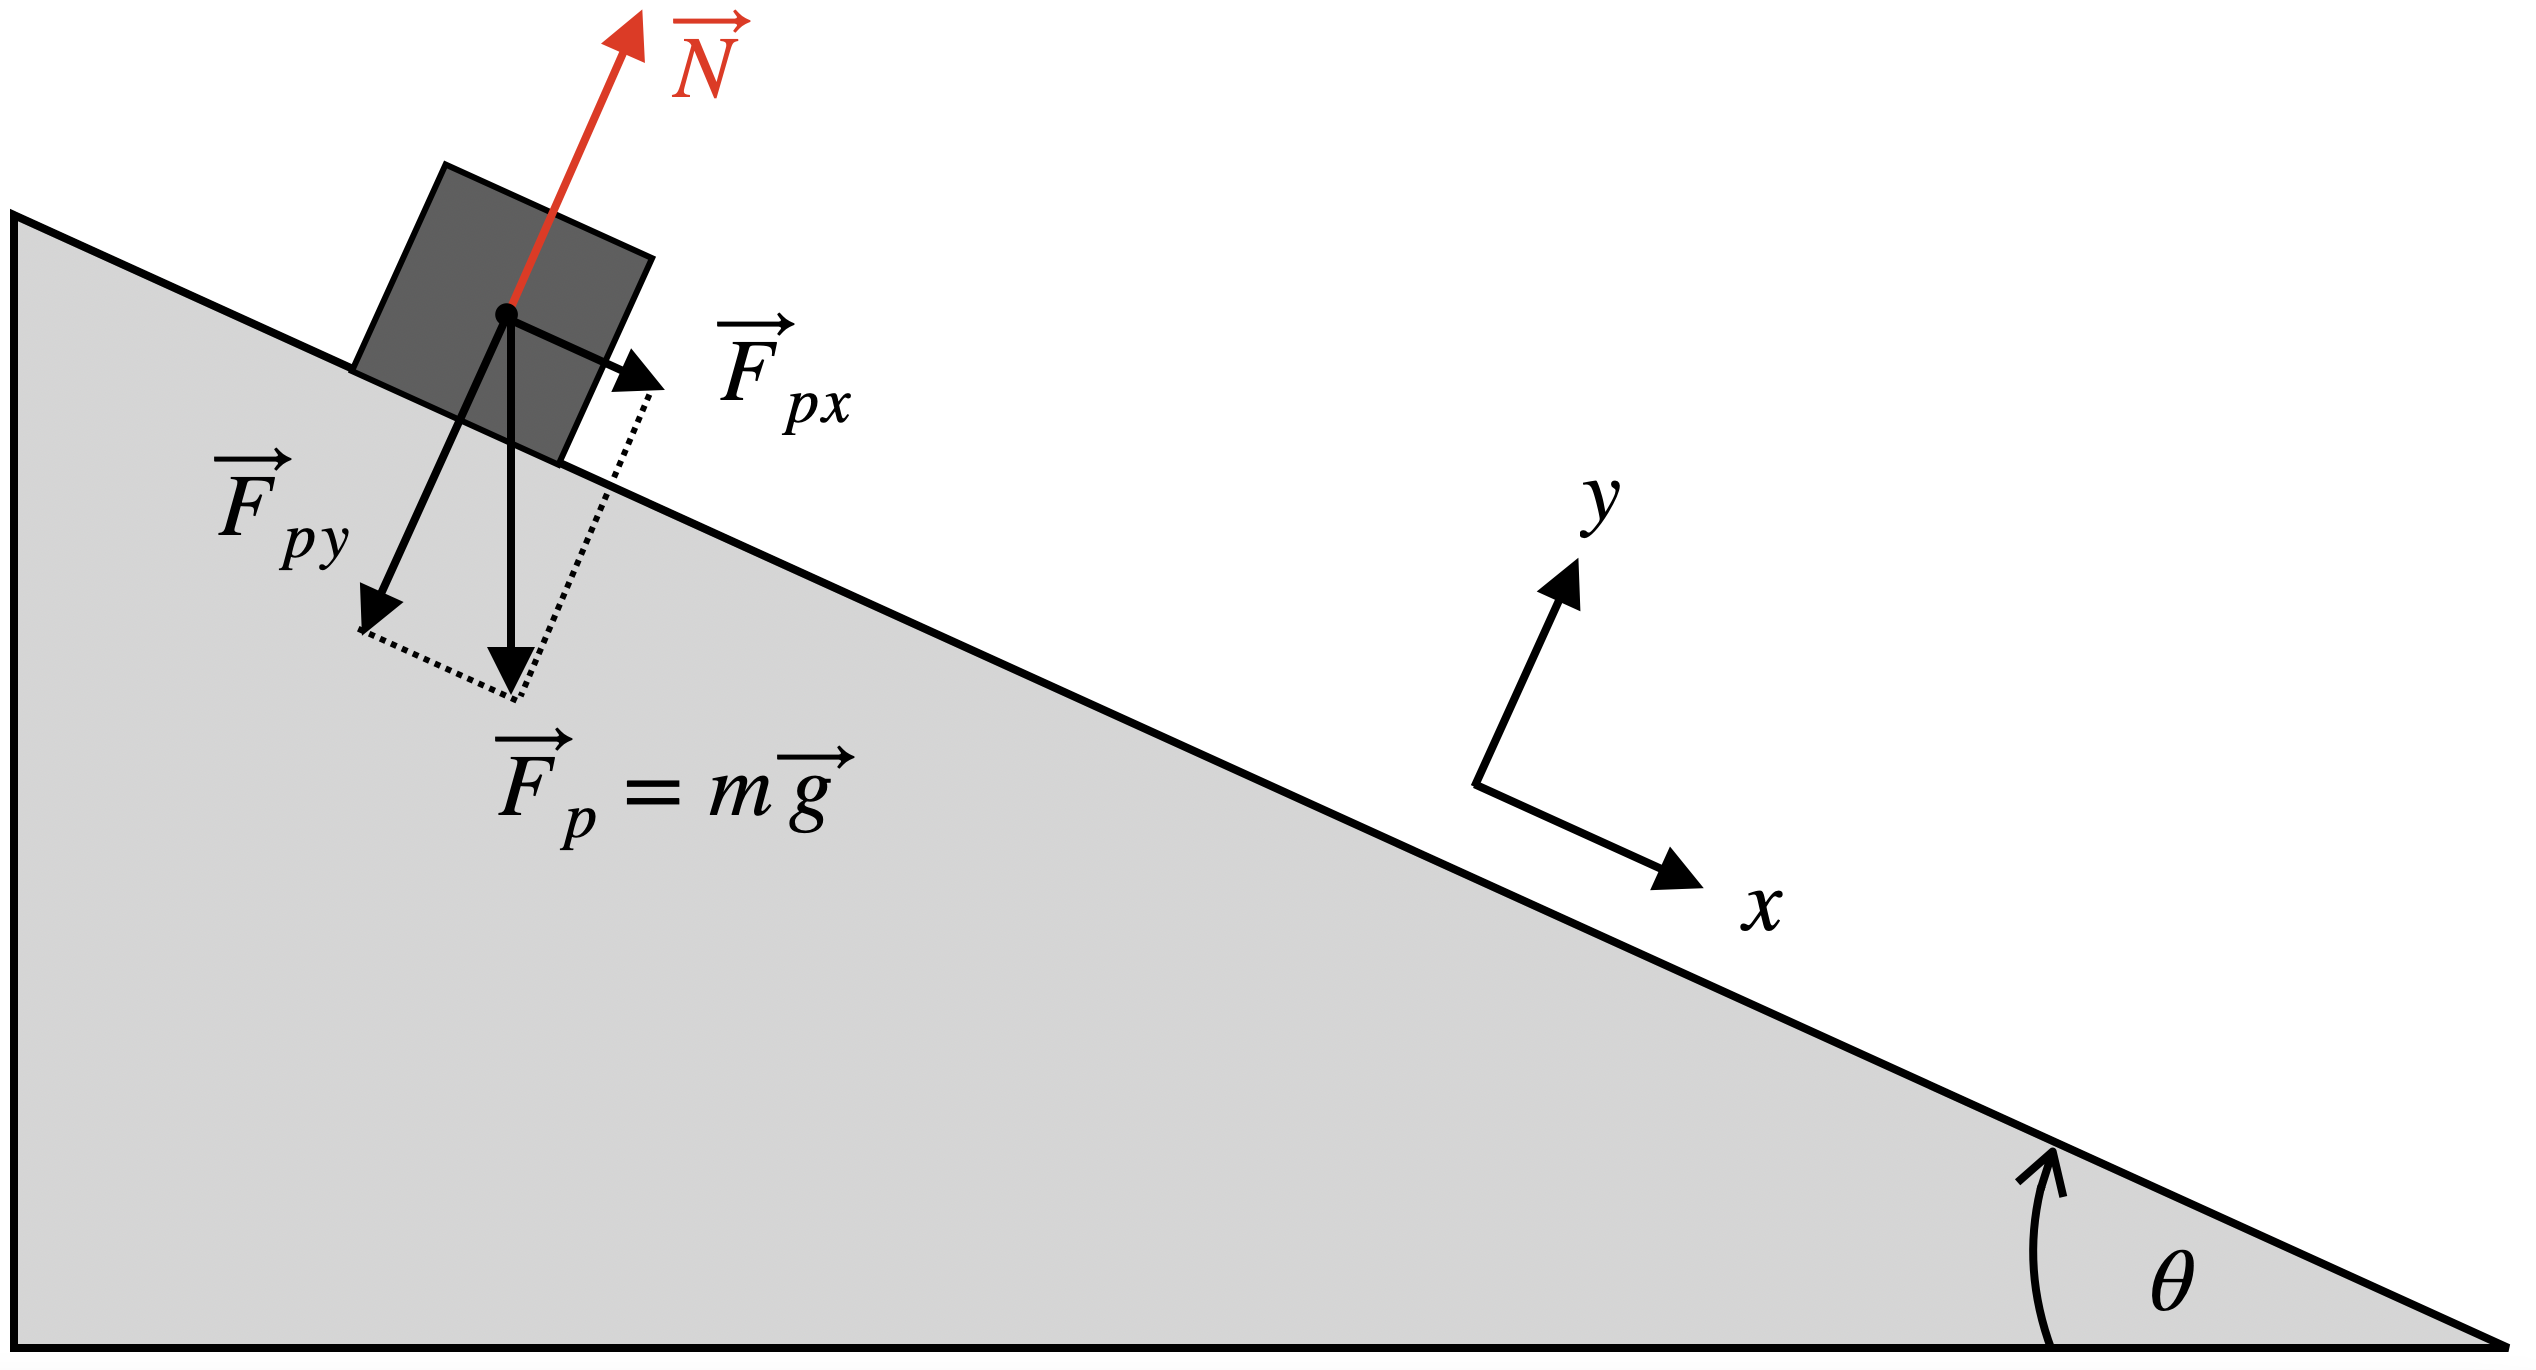
\includegraphics[width=10cm]{images/pianoincl.png}
        \caption{Rappresentazione di un piano inclinato con angolo $\theta$ e
        rappresentazione del sistema di riferimento scelto, con la coordinata $x$
        parallela al piano e la $y$ ortogonale.}
\end{center}
\label{fig:Iplain&pendulum:Iplain}
\end{figure}
\\
Nel caso con attrito avremo un moto solo se la componente parallela della
forza peso è maggiore della forza d'attrito massima:
\begin{equation}
    mg\sin\theta > \mu_s mg\cos\theta\seg \boxed{\tan\theta>\mu_s}
\end{equation}
Supponendo di trovarci in questa situazione, studiamo il caso dinamico:
\begin{equation}
    x:\quad mg\sin\theta -\mu_d mg\cos\theta = m\ddot x\seg
    \boxed{a_x = g\sx\sin\theta-\mu_d\cos\theta\dx}
\end{equation}
Dato che $\mu_d<\mu_s$, non può verificarsi il caso in cui $\tan\theta
=\mu_d$ che annullerebbe l'accelerazione lungo $x$.

\section{Pendolo semplice}
%---------------------------------------------------------------------------
\begin{figure}[htbp]
    \begin{center}
        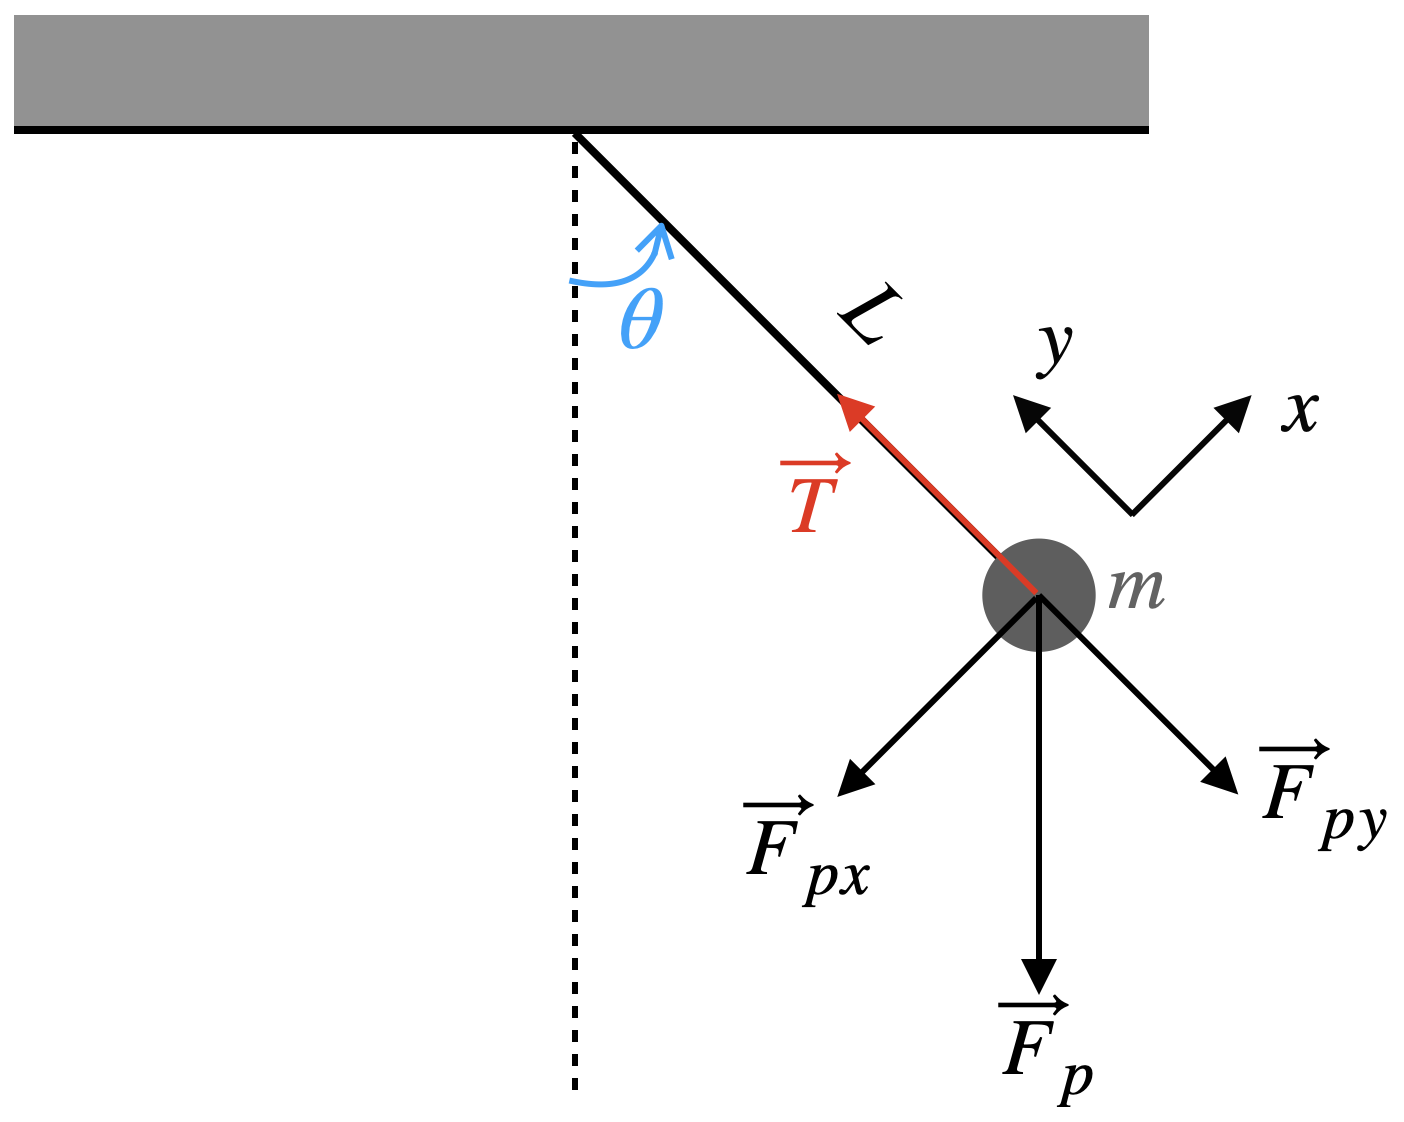
\includegraphics[width=10cm]{images/pendolo.png}
        \caption{Rappresentazione di un pendolo inclinato di un certo angolo
        $\theta$ rispetto alla verticale. È stato raffigurato anche il sistema
        di riferimento, con l'asse $y$ parallelo al filo di lunghezza $L$, e
        l'asse $x$ ortogonale ad esso.}
\end{center}
\label{fig:Iplain&pendulum:pendulum}
\end{figure}

Il pendolo è un sistema fisico costituito da un punto materiale di massa
$(m)$ sottoposto ad una forza costante, in questo caso la gravità, vincolato
ad avere una certa distanza $(L)$ da un punto fisso.\\
Nel caso mostrato in figura \ref{fig:Iplain&pendulum:pendulum}, la distanza
viene vincolata con un filo inestensibile teso con una tensione $(\vec T)$.
Vogliamo studiare la legge oraria dell'angolo $\theta$, l'angolo tra l'asse
verticale e la fune.\\
Scriviamo dunque le equazioni di Newton, considerando un asse parallelo alla
fune ed uno ortogonale.
\begin{equation}
    x:\quad -mg\sin\theta = ma_t\quad\quad y:\quad T-mg\cos\theta = ma_n
\end{equation}
\begin{equation}
    a_t = \frac{dv}{dt}=\frac d{dt}\sx L\dot\theta\dx=
    L\ddot\theta\quad\quad a_n = 0
\end{equation}
Lungo l'asse $y$ il corpo è in equilibrio, mentre lungo l'asse $x$ abbiamo
la seguente equazione differenziale:
\begin{equation}
    \boxed{\ddot\theta + \frac gL\sin\theta = 0}
\label{eq:pendulum_DE}
\end{equation}
Se consideriamo l'approssimazione di piccole oscillazioni, l'equazione differenziale appena ottenuta si riduce all'equazione dell'oscillatore armonico, in quanto:
\begin{equation}
    \theta \ll 1 \seg \sin\theta \sim \theta \seg
    \ddot\theta + \frac gL\theta = 0
\label{eq:pendulum_ODE}
\end{equation}
Dove la la pulsazione propria del sistema è $\omega_0 = \sqrt{\frac gL}$.
\begin{equation}
    \theta_{(t)} = \theta_0\sin\sx\omega_0t+\phi\dx\quad\quad
    \omega_{(t)} = \omega_0\theta_0\cos\sx\omega_0t+\phi\dx\quad\quad
    \theta_{(t)} =-\omega_0^2 \theta_0\sin\sx\omega_0t+\phi\dx
\end{equation}
\section{Lavoro ed Energia}
%---------------------------------------------------------------------------
Il lavoro di una è la quantità di energia scambiata tra due sistemi,
quando avviene uno spostamento per mezzo di una forza. Matematicamente è
definito come l'integrale della forza lungo una curva, ovvero il percorso
lungo cui si sposta il corpo.
\begin{equation}
    \boxed{W = \int_\gamma d\vec s \cdot \vec F}
\label{eq:work&energy:work_def}
\end{equation}
Ne segue che la forza è sempre ortogonale allo spostamento, questa non
compierà lavoro sul corpo. Se pensiamo ad $\vec F$ come una risultante
delle forze otterremo che:
\begin{equation}
    W =  \int_\gamma d\vec s \cdot \sum_{k=1}^n\vec F_k =
    \sum_{k=1}^n \int_\gamma d\vec s \cdot \vec F_k = \sum_{k=1}^n W_k
\label{eq:work&energy:work_sum}
\end{equation}
Il lavoro totale può essere visto come la somma dei lavori delle singole
forze che costituiscono $\vec F$.
Se il lavoro è positivo, allora di dice lavoro motore, mentre se è negativo
si dice lavoro resistente.
Il lavoro essendo un'energia è misurato nel S.I. con il $(J)$ Joule.
Un Joule è definito come l'energia scambiata da una forza di un Newton, per
compiere uno spostamento di un metro lungo la sua stessa direzione:
$1J = 1N\cdot 1 m$. 
\subsection{Potenza}
La potenza esprime la velocità con cui viene trasferita una particolare forma
di energia. Adesso parleremo di potenza meccanica, definita come la derivata
rispetto al tempo del lavoro, ed è misurata in Watt $(W)$.
Una potenza di un Watt trasferisce un Joule in un secondo.
\begin{equation}
    \boxed{P=\frac{dW}{dt}}
\label{eq:work&energy:power_def}
\end{equation}
\subsection{Lavoro come variazione di energia cinetica}
Scriviamo il lavoro infinitesimo per una forza generica data da
$\vec F = m\vec a$.
\begin{equation}
    dW = \vec F\cdot d\vec s = ma_tds = m\dot v ds = mv dv 
\end{equation}
Integrando otterremo che il lavoro per spostare il corpo dal punto $A$ al
punto $B$ sarà:
\begin{equation}
    W = \int_{v_A}^{v_B}mvdv = \frac12mv_B^2- \frac12mv_A^2
\end{equation}
Quindi definendo l'energia cinetica, l'energia associata al movimento di un
corpo, come $K = \frac12 mv^2=\frac{p^2}{2m}$, otteniamo che:
\begin{equation}
    W = K_B - K_A = \Delta K
\label{eq:work&energy:w=dk}
\end{equation}
\subsection{Lavoro della forza gravitazionale}
Prendiamo il caso in cui la forza peso faccia spostare un corpo di massa $m$
da un punto $A$ ad un punto $B$, a quota più bassa di $A$. Supponiamo che il corpo segua un percorso a piacere, purché vada da $A$ a $B$. quindi prendo un asse verticale $z$ diretto verso l'alto, otterremo che:
\begin{figure}[htbp]
    \begin{center}
        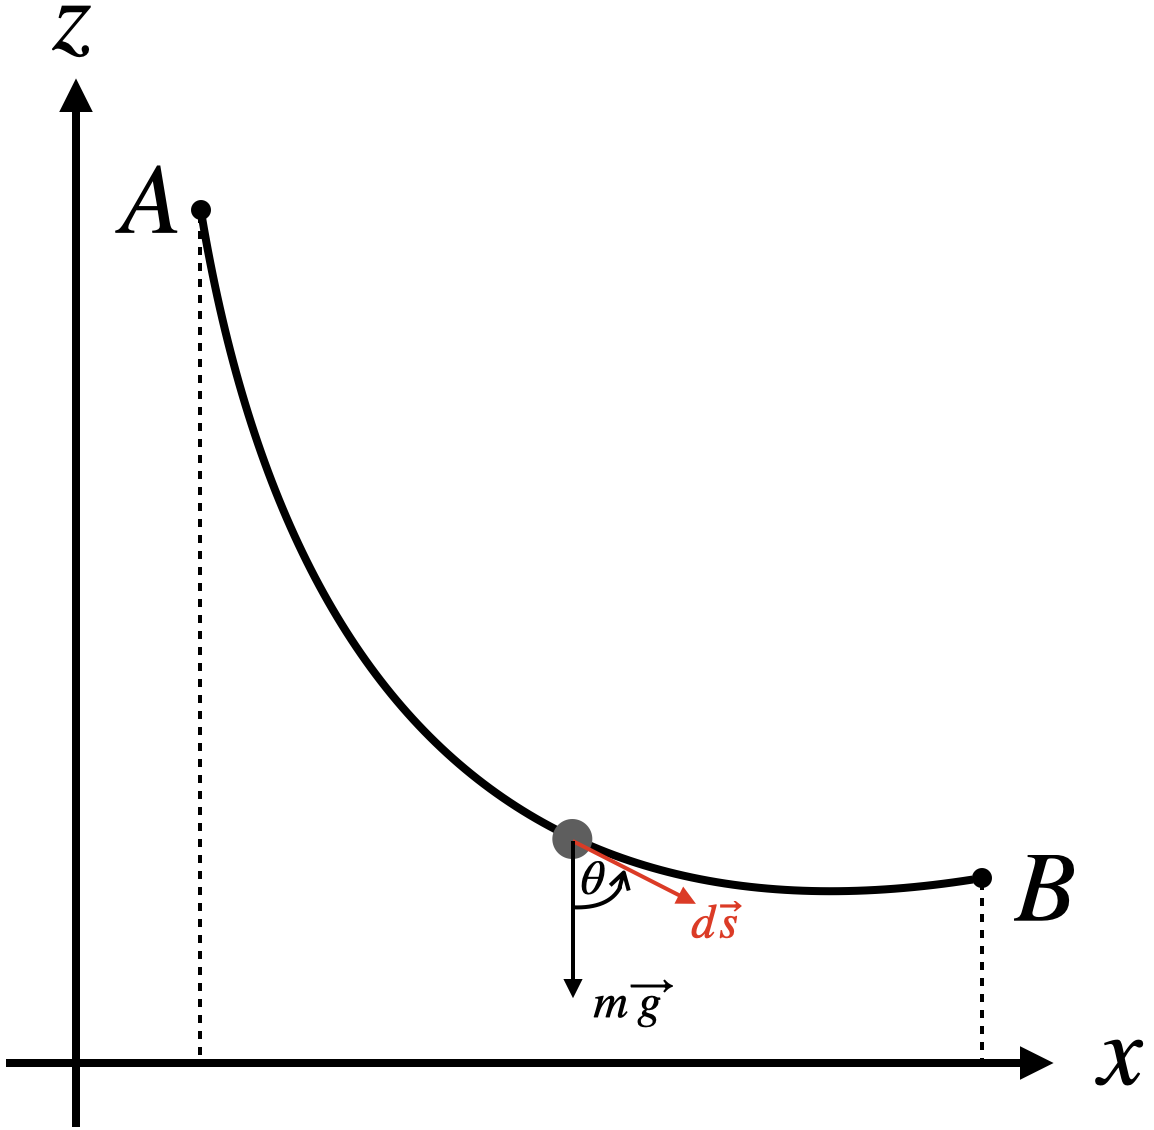
\includegraphics[width=10cm]{images/lavorog.png}
        \caption{Rappresentazione del lavoro infinitesimo lungo un tratto
        elementare di curva $d\vec s$ del forza gravitazionale
        $\vec F_p = m\vec g$.}
\end{center}
\label{fig:work&energy:P_work}
\end{figure}

\begin{equation}
    W = \int_A^Bd\vec s \cdot\vec F_p = -mg\int_A^Bds\cos\theta =
    -mg\int_A^Bdz = -mg\sx z_B-z_A\dx
\end{equation}
Ovvero definendo l'energia potenziale gravitazionale come $U = mgz$, abbiamo
che il lavoro è meno la variazione di energia potenziale:
\begin{equation}
    W = U_A-U_B = -\Delta U
\label{eq:work&energy:w=-du}
\end{equation}
imponendo uguali le equazioni $(2.48)$ e $(2.50)$ otteniamo il principio di
conservazione dell'energia meccanica $E = K + U$.
\begin{multline}
    \Delta K = -\Delta U\seg K_B-K_A = U_A -U_B\seg
    \\\seg K_A+U_A = K_B+U_B\seg
    \boxed{E_A = E_B}
\end{multline}
\subsection{Lavoro della forza elastica}
Calcoliamo il lavoro di una forza elastica diretta lungo
$x$: $\vec F_e = -kx\hat\imath$.
\begin{equation}
    W = -k\int_A^Bdx x = \frac12 kx_A^2-\frac12 kx^2_B\quad\quad
    U_e = \frac12 kx^2\seg W = -\Delta U_e
\label{eq:work&energy:elastic_energy}
\end{equation}
\subsection{Lavoro della forza d'attrito radente}
La forza d'attrito, essendo sempre diretta in verso opposto alla velocità
produce un lavoro negativo, ovvero sempre resistente. L'integrale sulla
curva dipende dal percorso scelto, al contrario delle forze conservative,
e quindi in un percorso chiuso il lavoro d'attrito sarà diverso da zero.
\begin{equation}
    \vec F_a = -\mu_d N \hat u_v\seg W_a = -\mu_d\int_A^BdsN =
    -\mu_dN\Delta s
    \label{eq:work&energy:work_friction}
\end{equation}
\subsection{Lavoro di forze conservative e non conservative}
Come abbiamo visto, il lavoro di una forza conservativa, che ammette
un'energia potenziale, non dipende dal percorso su cui si integra, ne segue
che se scegliamo un percorso chiuso l'integrale sulla curva chiusa sarà
sempre nullo.\\
Quindi se $\vec F$ è una forza conservativa ne segue che:
\begin{equation}
    \boxed{\oint_\gamma d\vec s \cdot F = 0}
\label{eq:work&energy:conservative_force}
\end{equation}
Dunque in questi casi che l'energia meccanica si conserva, quindi l'energia
meccanica nello stato iniziale è uguale all'energia meccanica nello stato
finale:
\begin{equation}
    \boxed{E_i = E_f}
\label{eq:work&energy:Ei=Ef}
\end{equation}
Mentre nel caso in cui sono presenti forze non conservative, il lavoro delle
forze non conservative non è nullo ed è pari alla variazione di energia
meccanica. E dato che durante il processo si dissipa energia:
\begin{equation}
    \boxed{W_{NC} = \Delta E = E_f- E_i < 0}
\label{eq:work&energy:Ei>Ef}
\end{equation}
Se prendiamo una generica forza $\vec F_{\sx x,y,z\dx} = \sx F_x,F_y,F_z\dx$,
se supponiamo che essa sia conservativa possiamo scrivere che:
\begin{equation}
    \int_A^Bd\vec s\cdot \vec F = \int F_xdx+F_ydy+F_zdz
\end{equation}
Ora se ammettiamo l'esistenza di un'energia potenziale, tale per cui la forza
è il suo gradiente cambiato di segno:
\begin{equation}
    \vec F_{\sx x,y,z\dx} = -\vec\nabla U_{\sx x,y,z\dx} = -\sx\frac{\partial U}{\partial x},\frac{\partial U}{\partial y},\frac{\partial U}{\partial z}\dx
\label{eq:work&energy:gradient}
\end{equation}
Trovandoci in questa situazione avremo che:
\begin{equation}
    \int_A^B F_xdx+F_ydy+F_zdz = -\int\vec \nabla U\cdot d\vec x = -\int dU = -\sss U_{(B)}-U_{(A)}\ddd = -\Delta U
\end{equation}
Come possiamo notare i risultati ottenuti nelle equazioni (\ref{eq:work&energy:w=-du})
e (\ref{eq:work&energy:elastic_energy}),sono in realtà molto più generali e,
data una forza esprimibile come il gradiente di un'energia potenziale
(cambiato di segno), si avrà che il lavoro da un punto $A$ a un punto $B$
seguendo una qualsiasi curva, sarà pari a meno la variazione di energia
potenziale. Di conseguenza una volta appreso queso fatto, possiamo capire
facilmente il perchè dell'equazione (\ref{eq:work&energy:conservative_force}).
Se si sceglie una curva chiusa, punto $A$ coincide con il punto $B$ dunque
dato che l'energia potenziale iniziale e finale sono uguali, il lavoro è
nullo.\\
Sotto le ipotesi di forze conservative si può dimostrare facilmente l'equazione
\ref{eq:work&energy:Ei=Ef}, ovvero la conservazione dell'energia meccanica.
\begin{equation}
    \frac{dE}{dt} = \frac12m\frac{d}{dt}v^2+\frac{dU}{dt} =
    \vec v\cdot m\frac{d\vec v}{dt} + \frac{d\vec x}{dt}\cdot\vec\nabla U =
    \vec v\sx m\vec a + \vec\nabla U\dx = 0
\label{eq:work&energy:energy_conservation}
\end{equation}
\section{Momento angolare}
%---------------------------------------------------------------------------
Il momento angolare è una grandezza molto importante in fisica, esso è
definito come il prodotto vettoriale tra il raggio vettore ed il vettore
impulso. È analogo alla quantità di moto in quanto, infatti esprime un
concetto di resistenza non al cambio di velocità lineare come nel caso
dell'impulso, ma al cambiamento dello stato di rotazione di un corpo.
Infatti se un corpo ha un momento angolare costante nel tempo, allora si
muove di moto circolare uniforme. Mentre se il momento angolare varia nel
tempo, esisterà un'accelerazione angolare.
\begin{equation}
    \boxed{\vec L = \vec r \times \vec p = \vec r \times m\vec v}
\label{eq:momentum:L_def}
\end{equation}
È importante ricordare che il momento angolare è uno pseudo-vettore in quanto
ha una forma diversa in base al polo rispetto al quale viene calcolato.
Ad esempio se trasliamo l'origine degli assi $O$ in $O'$, come mostrato in
figura (\ref{fig:momentum:pole_change}), otterremo che:
\begin{equation}
    \vec L = \vec r \times \vec p\quad \quad \vec L' = \vec r '\times\vec p =
    \sx\vec r + \vec t\dx\times \vec p = \vec r \times \vec p + \vec t\times
    \vec p = \vec L + \vec t\times\vec p
\end{equation}
Quindi traslando il polo otterremo una variazione del momento angolare che è
la seguente:
\begin{equation}
    \boxed{\vec L'-\vec L = \vec t\times\vec p}
\label{eg:momentum:L_pole_change}
\end{equation}
\begin{figure}[htbp]
    \begin{center}
        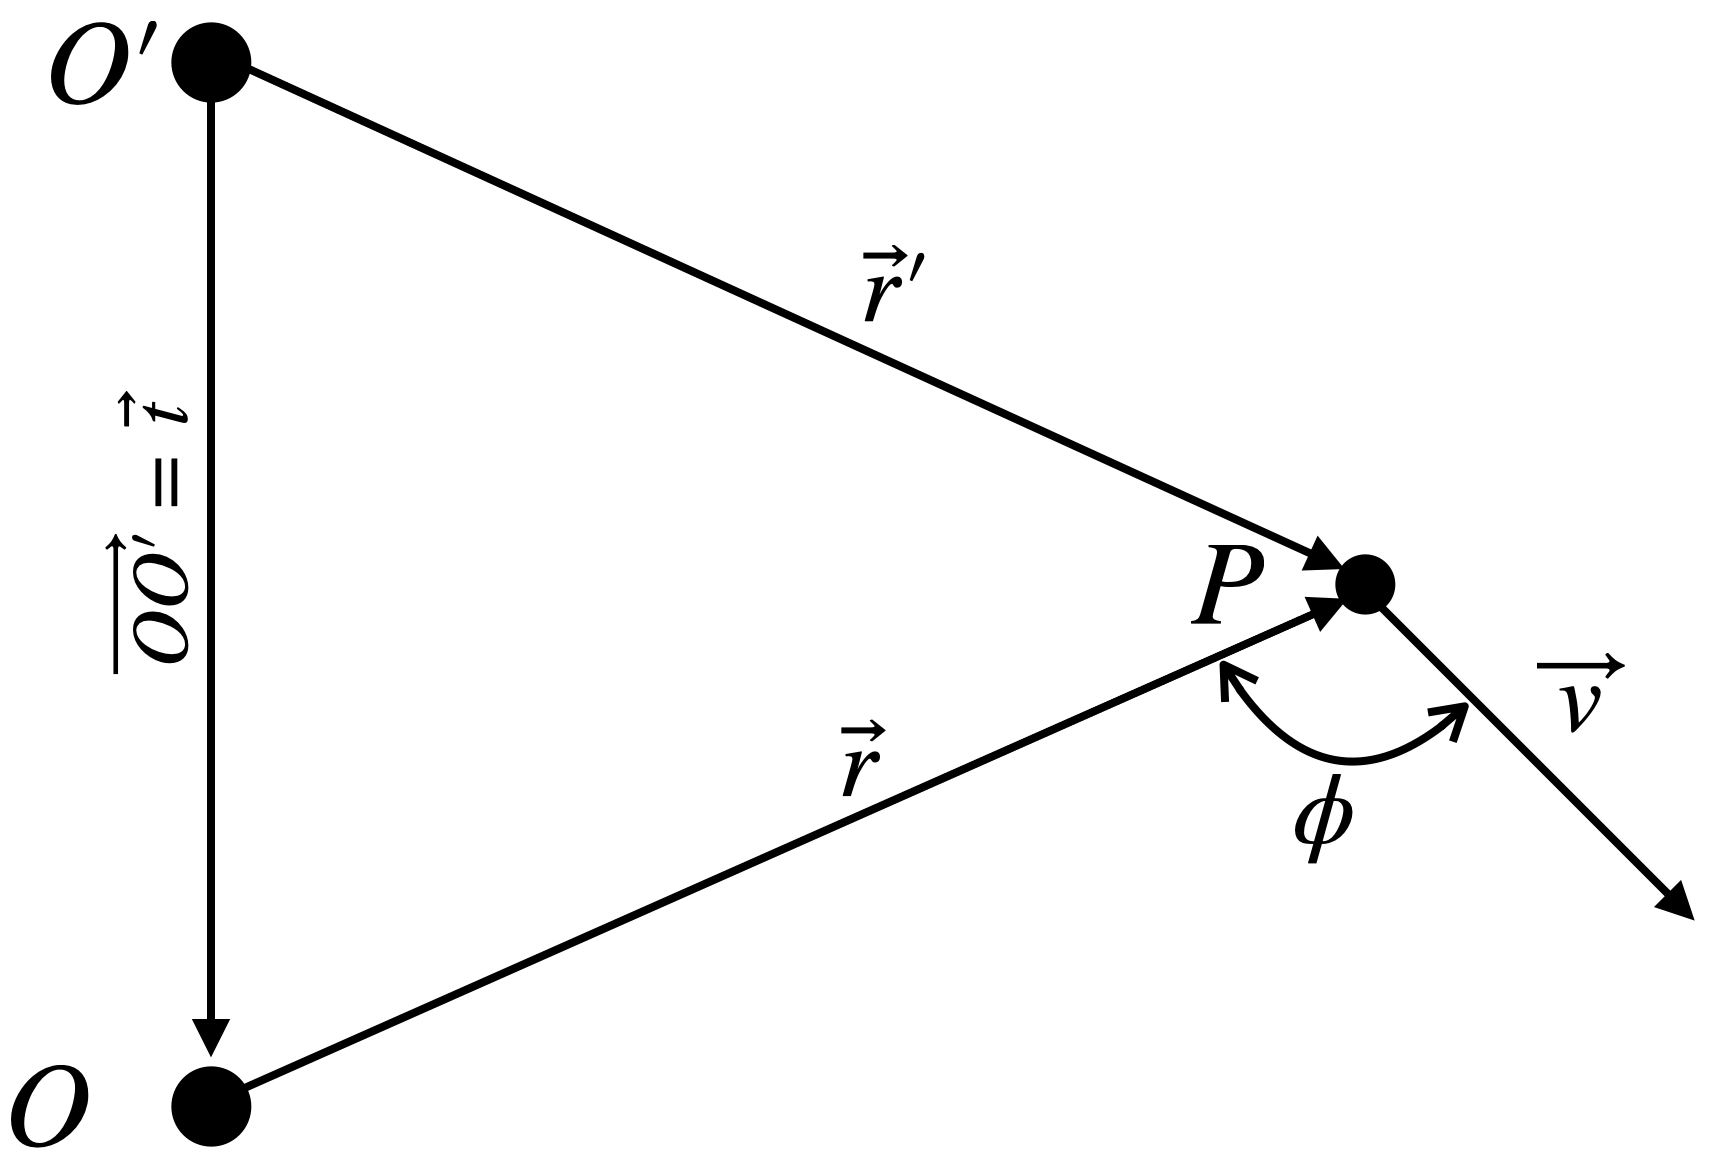
\includegraphics[width=10cm]{images/momang1.png}
        \caption{Schema dei vettori $\vec r$, $\vec r'$, $\vec v$ e $\vec t$,
        utilizzati per il calcolo del momento angolare rispetto ai poli $O$ ed
        $O'$.}
\label{fig:momentum:pole_change}
\end{center}
\end{figure}
\\
In coordinate polari possiamo scrivere la velocità come somma della sua
componente radiale e quella trasversa, ne segue che dato che la componente
radiale è parallela al raggio vettore, essa non da contributo al momento
angolare.
\begin{equation}
    \vec L = \vec r \times m\sx \vec v_r+\vec v_\phi\dx = \vec r \times m\vec v_\phi
\end{equation}
Quindi dato che $\vec v_\phi = r\frac{d\phi}{dt}\hat\phi$ possiamo scrivere il modulo
del momento angolare di un punto materiale nel seguente modo:
\begin{equation}
    \boxed{L = mr^2\frac{d\phi}{dt} = I\omega}
\label{eq:momentum:l=Iw}
\end{equation}
Dove abbiamo chiamato $I$ il momento d'inerzia. Il momento d'inerzia è un
analogo del termine di massa che compare nella definizione di impulso,
quindi come la massa esprime un concetto di resistenza alla variazione dello
stato di moto, il momento d'inerzia rappresenta lo stesso concetto, ma per
moti rotatori. Da notare dunque l'analogia in formule:
$\vec p$ con $\vec L$, $m$ con $I$ e $\vec v$ con $\vec \omega$.
\begin{equation}
\vec p = m\vec v \quad\quad \quad \vec L = I\vec\omega
\end{equation} 
In questo caso il momento d'inerzia di un punto che ruota su una
circonferenza di raggio $r$ è pari ad $I = mr^2$. Vedremo poi in seguito,
nel capitolo sui corpo rigidi, come in realtà questo momento d'inerzia per
corpo estesi è una matrice, dunque in generale potremmo incontrare casi in
cui il momento angolare non è parallelo alla velocità angolare.
\section{Momento di una forza}
%---------------------------------------------------------------------------
In analogia con il momento angolare, il momento di una forza è definito dal
prodotto vettoriale tra il raggio vettore e la forza.
\begin{equation}
    \boxed{\vec M = \vec r \times \vec F}
\label{eq:momentum:M_def}
\end{equation}
Partendo dalla definizione di momento angolare, si può effettuare la derivata
rispetto al tempo ottenendo infine la relazione che lega momento angolare e
momento delle forze.
\begin{equation}
    \vec L = \vec r \times \vec p \seg \frac{d\vec L}{dt} =
    \cancel{\vec v\times\vec p} + \vec r \times \frac{d\vec p}{dt} \seg
    \boxed{\vec M = \frac{d\vec L}{dt}}
\label{eq:momentum:M=dot_L}
\end{equation}
\subsection{Teorema dell'impulso angolare}
Analogamente a quanto fatto per il teorema dell'impulso, iniziamo integrando
l'equazione (\ref{eq:momentum:M=dot_L}).
\begin{equation}
    \vec M = \frac{d\vec L}{dt} \seg \int_0^\tau dt\frac{d\vec L}{dt} = \int_0^\tau dt \vec M \seg \Delta \vec L =\int_0^\tau dt \vec M 
\end{equation}
\begin{equation}
    \vec{M_m} = \frac1\tau\int_0^\tau dt \vec M = \frac{\Delta \vec L}{\tau}
\end{equation}